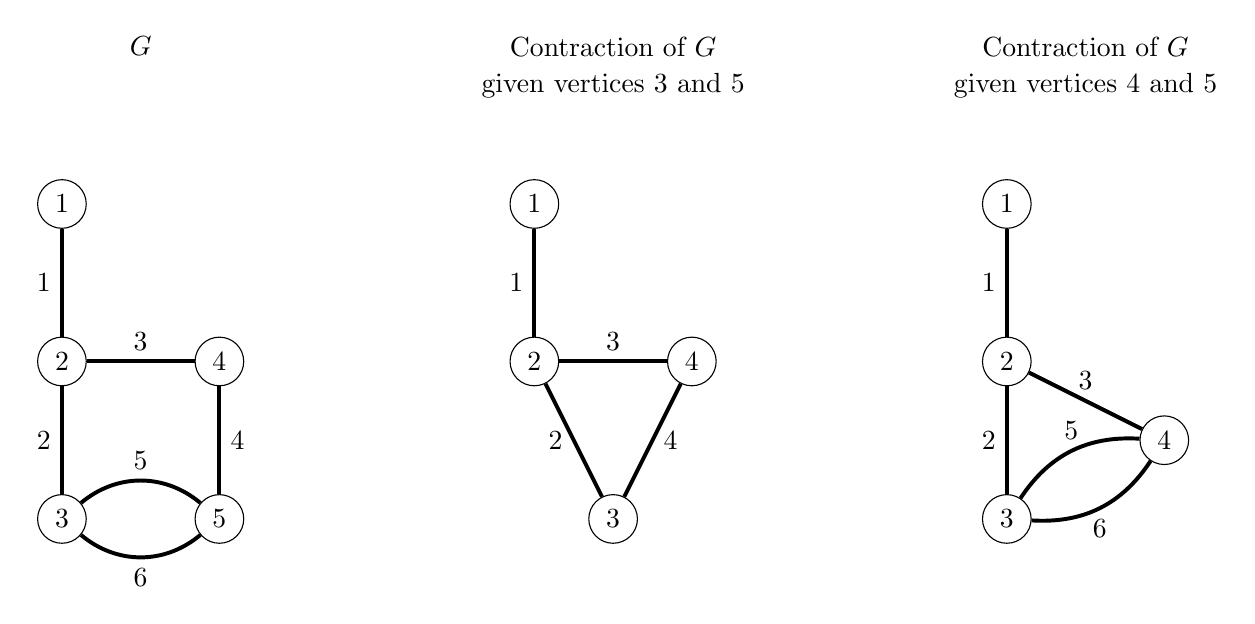
\begin{tikzpicture}
	\begin{scope}[xshift=0cm, yshift=0cm]
		\node (G) at (1, 6) {$G$};

		\node[circle, draw] (1) at (0, 4) {1};
		\node[circle, draw] (2) at (0, 2) {2};
		\node[circle, draw] (3) at (0, 0) {3};
		\node[circle, draw] (4) at (2, 2) {4};
		\node[circle, draw] (5) at (2, 0) {5};
	
		% Draw the edges between nodes with labels
		\draw[line width=0.5mm] (1) -- node[left] {1} (2);
		\draw[line width=0.5mm] (2) -- node[left] {2} (3);
		\draw[line width=0.5mm] (2) -- node[above] {3} (4);
		\draw[line width=0.5mm] (4) -- node[right] {4} (5);
		\draw[line width=0.5mm] (3) to[bend left=40] node[above] {5} (5);
		\draw[line width=0.5mm] (3) to[bend right=40] node[below] {6} (5);
	\end{scope}
	
	\begin{scope}[xshift=6cm, yshift=0cm]
		\node (G) at (1, 6) {Contraction of $G$};
		\node (G) at (1, 5.5) {given vertices 3 and 5};

		\node[circle, draw] (1) at (0, 4) {1};
		\node[circle, draw] (2) at (0, 2) {2};
		\node[circle, draw] (3) at (1, 0) {3};
		\node[circle, draw] (4) at (2, 2) {4};
	
		% Draw the edges between nodes with labels
		\draw[line width=0.5mm] (1) -- node[left] {1} (2);
		\draw[line width=0.5mm] (2) -- node[left] {2} (3);
		\draw[line width=0.5mm] (2) -- node[above] {3} (4);
		\draw[line width=0.5mm] (4) -- node[right] {4} (3);
	\end{scope}

	\begin{scope}[xshift=12cm, yshift=0cm]
		\node (G) at (1, 6) {Contraction of $G$};
		\node (G) at (1, 5.5) {given vertices 4 and 5};

		\node[circle, draw] (1) at (0, 4) {1};
		\node[circle, draw] (2) at (0, 2) {2};
		\node[circle, draw] (3) at (0, 0) {3};
		\node[circle, draw] (4) at (2, 1) {4};
	
		% Draw the edges between nodes with labels
		\draw[line width=0.5mm] (1) -- node[left] {1} (2);
		\draw[line width=0.5mm] (2) -- node[left] {2} (3);
		\draw[line width=0.5mm] (2) -- node[above] {3} (4);
		\draw[line width=0.5mm] (3) to[bend left=30] node[above] {5} (4);
		\draw[line width=0.5mm] (3) to[bend right=30] node[below] {6} (4);
	\end{scope}
\end{tikzpicture}
